%
% Beispielkapitel: Bedienung dieser Vorlage
%

% Zum Setzen von TeX-Quellcode, der nicht interpretiert werden soll
\newcommand{\makro}[1]{\texttt{\textbackslash{}#1\{\}}}

\chapter{Overview}
\label{sec:overview}

The following chapter will give a quick overview of the hard- and software which is currently used on the remote-controlled car. The whole system can be seen in picture \ref{fig:rccar_overview}

\begin{figure}[h]
	\centering
		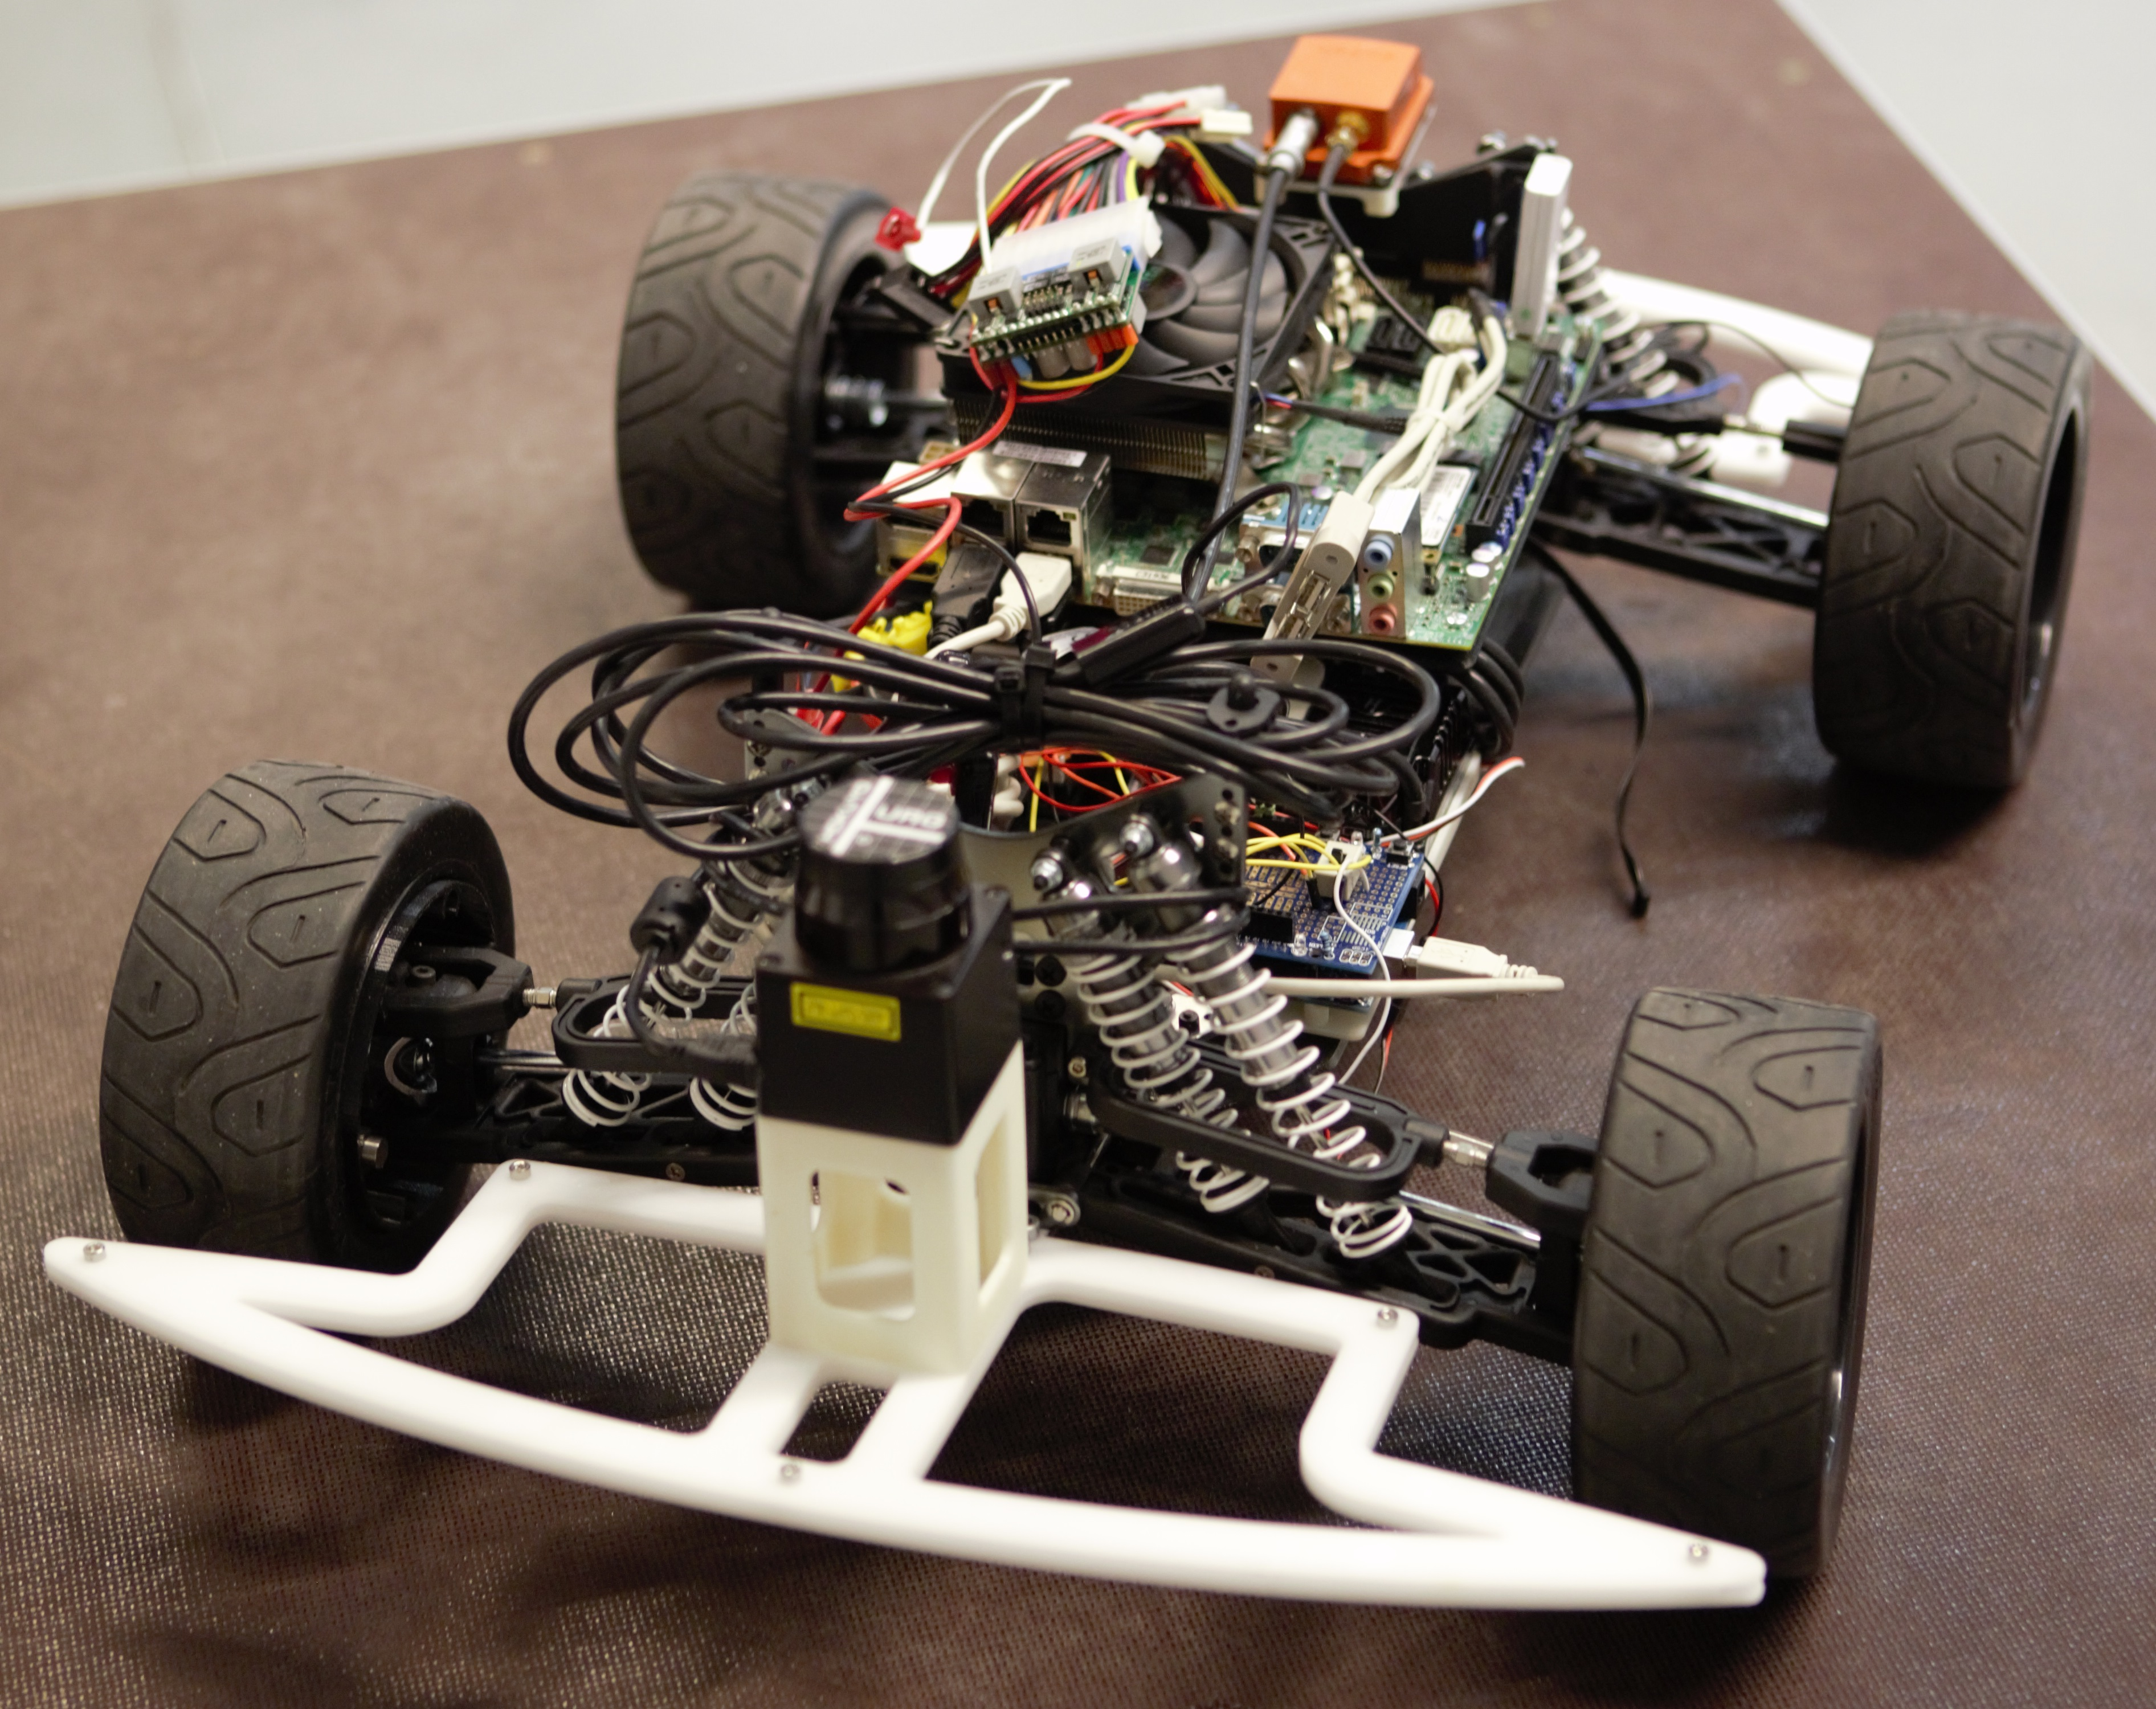
\includegraphics[width=\textwidth]{car}
	\caption{Picture of the rc-car}
	\label{fig:rccar_overview}
\end{figure}


\newpage
%=========================================================================================
\section{Hardware}
%=========================================================================================
\label{sec:overview_hardware}

This section will give a short introduction to the hardware which can be found on the car.

%=========================================================================================
\subsection{Motors and controllers}
\label{sec:overview_motors}

On the car we can find two electrical motors, one for driving the car and one for the steering. 

\begin{figure}[h]
	\centering
		\includegraphics[width=0.5\textwidth]{brushless_motor}
	\caption{HACKER Skalar 8 brushless motor}
	\label{fig:brushless_motor}
\end{figure}


In picture \reffig{brushless_motor} we can see the electrical brushless motor which is used to drive the wheels.The motor is connected to the wheels over a gear and two differentials. Table \reftab{motor_details} gives some details of the used type. More information can be found here:

\hyperref[http://www.hacker-carline.de/produkte/skalar-motoren/hacker-skalar-10/]{http://www.hacker-carline.de/produkte/skalar-motoren/hacker-skalar-10/}

\begin{table}[b]
	\centering	
	\begin{tabular}{cc} % eine Tabelle mit drei Spalten, in denen der Text jeweils zentriert ist
		\hline 
		Name: & HACKER Skalar 8 1750 \\
		max. Power (W): & 1650 \\
		max. RPM (1/min): & 25900 \\
		max. voltage (V): & 14.8 \\
		max. current (A): & 110 \\
		\hline
	\end{tabular}
	\caption{Hacker Skalar 8 - Details} % Die Beschriftung der Tabelle
	\label{tab:motor_details}
\end{table}


For steering, there is a second motor at the front of the car.

Both motors bring its own controllers which take a PWM-signal as input to set the desired revolution rate or angle. The principal is shown in picture \reffig{pwm_signals}. Both input signals are provided by a little Arduino board (see next section 1.1.2).

\begin{figure}[h]
	\centering
		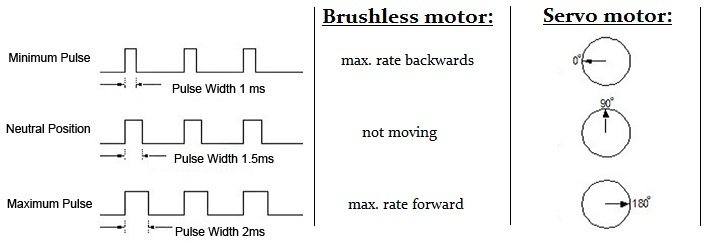
\includegraphics[width=\textwidth]{pwm_signals}
	\caption{PWM-signals for the motors}
	\label{fig:pwm_signals}
\end{figure}


\subsection{Arduino board}
\label{sec:overview_arduino}
\begin{figure}[h]
	\centering
		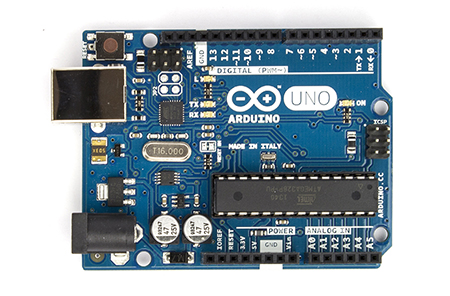
\includegraphics[width=0.35\textwidth]{arduino}
	\caption{Arduino UNO board}
	\label{fig:arduino}
\end{figure}

To provide the signals to the motor controllers there is a little Arduino UNO board on the car which can be seen in picture \reffig{arduino}. It receives the PWM-values from the mainboard of the car via USB and sets them to the output pins which are connected to the controllers.

\subsection{Linux-Board}
\label{sec:overview_board}

For computing there is a Supermicro X10SLV motherboard with a Intel Core i7 processor on it. To control the system we use Ubuntu 14.04 and a special software framework called ROS (see section \refsec{overview_software}). Table \ref{tab:computer_details} gives a short overview of the computer system. More information can be found on:

\hyperref[http://www.supermicro.com/products/motherboard/Core/H81/X10SLV.cfm]{http://www.supermicro.com/products/motherboard/Core/H81/X10SLV.cfm}

\begin{table}[h]
	\centering	
	\begin{tabular}{cc} % eine Tabelle mit drei Spalten, in denen der Text jeweils zentriert ist
		\hline 
		Motherboard: & Supermicro X10SLV \\
		Processor: & Intel Core i7 8 x 3GHz \\
		Memory: & 16GB DDR3 \\
						& 128GB Flash memory \\
		\hline
	\end{tabular}
	\caption{Computer system - Details} % Die Beschriftung der Tabelle
	\label{tab:computer_details}
\end{table}

\newpage
\subsection{Laserscanner}
\label{sec:overview_laserscanner}

\begin{figure}[h]
	\centering
		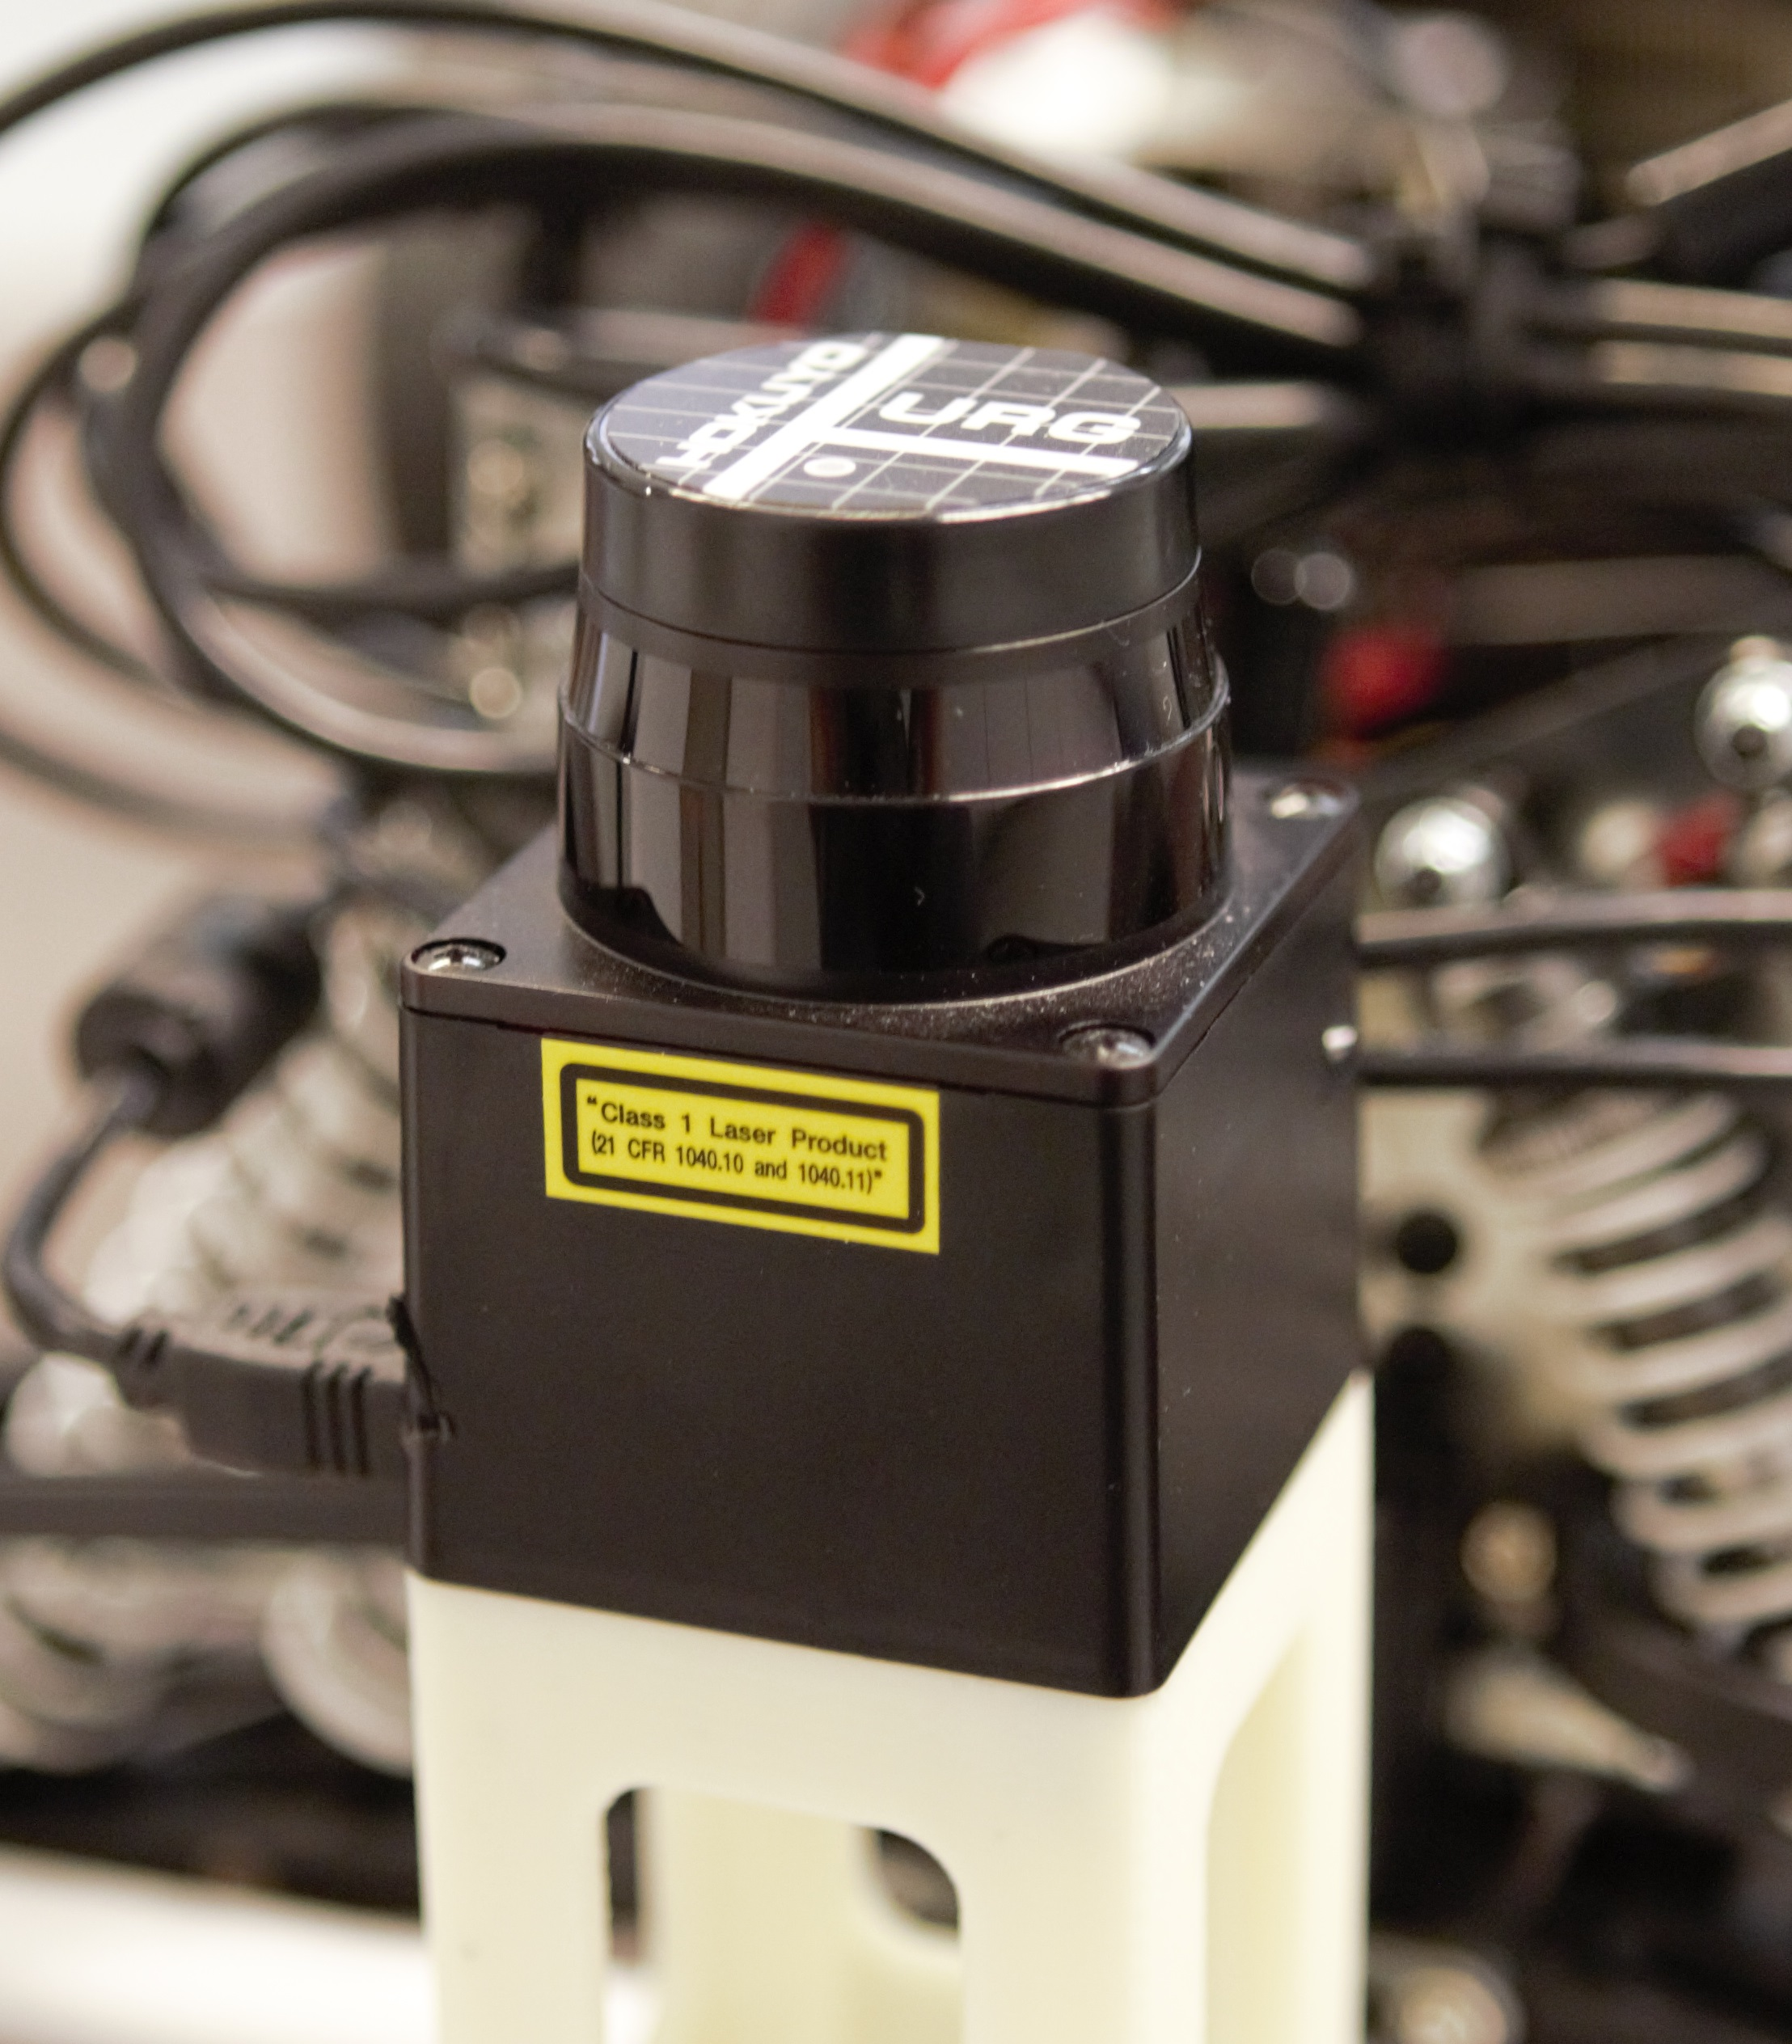
\includegraphics[width=0.35\textwidth]{hokuyo_urg_04lx}
	\caption{Hokuyo URG-04LX-UG01}
	\label{fig:hokuyo}
\end{figure}

At the front of the car we can find a Hokuyo URG-04LX-UG01 laserscanner (see picture \reffig{hokuyo}). The scanner is used for location in a given 2-D map or to create maps while the car is moving through the environment. For detailed information about the scanner refer to:

\hyperref[https://www.hokuyo-aut.jp/02sensor/07scanner/urg_04lx_ug01.html]{https://www.hokuyo-aut.jp/02sensor/07scanner/urg\_04lx\_ug01.html}

\begin{table}[h]
	\centering	
	\begin{tabular}{cc} % eine Tabelle mit drei Spalten, in denen der Text jeweils zentriert ist
		\hline 
		Name: & Hokuyo URG-04LX-UG01 \\
		Measuring area: & 20 to 5600mm(white paper with 70mm×70mm), 240\textdegree \\
		Accuracy: & 60 to 1,000mm : ±30mm, \\
							&	1,000 to 4,095mm : ±3 percent of measurement \\
		Scanning time & 100ms/scan \\
		\hline
	\end{tabular}
	\caption{Laserscanner - Details} %
	\label{tab:laser_details}
\end{table}


\newpage
\subsection{Inertial measurement unit (IMU)}
\label{sec:overview_imu}

\begin{figure}[h]
	\centering
		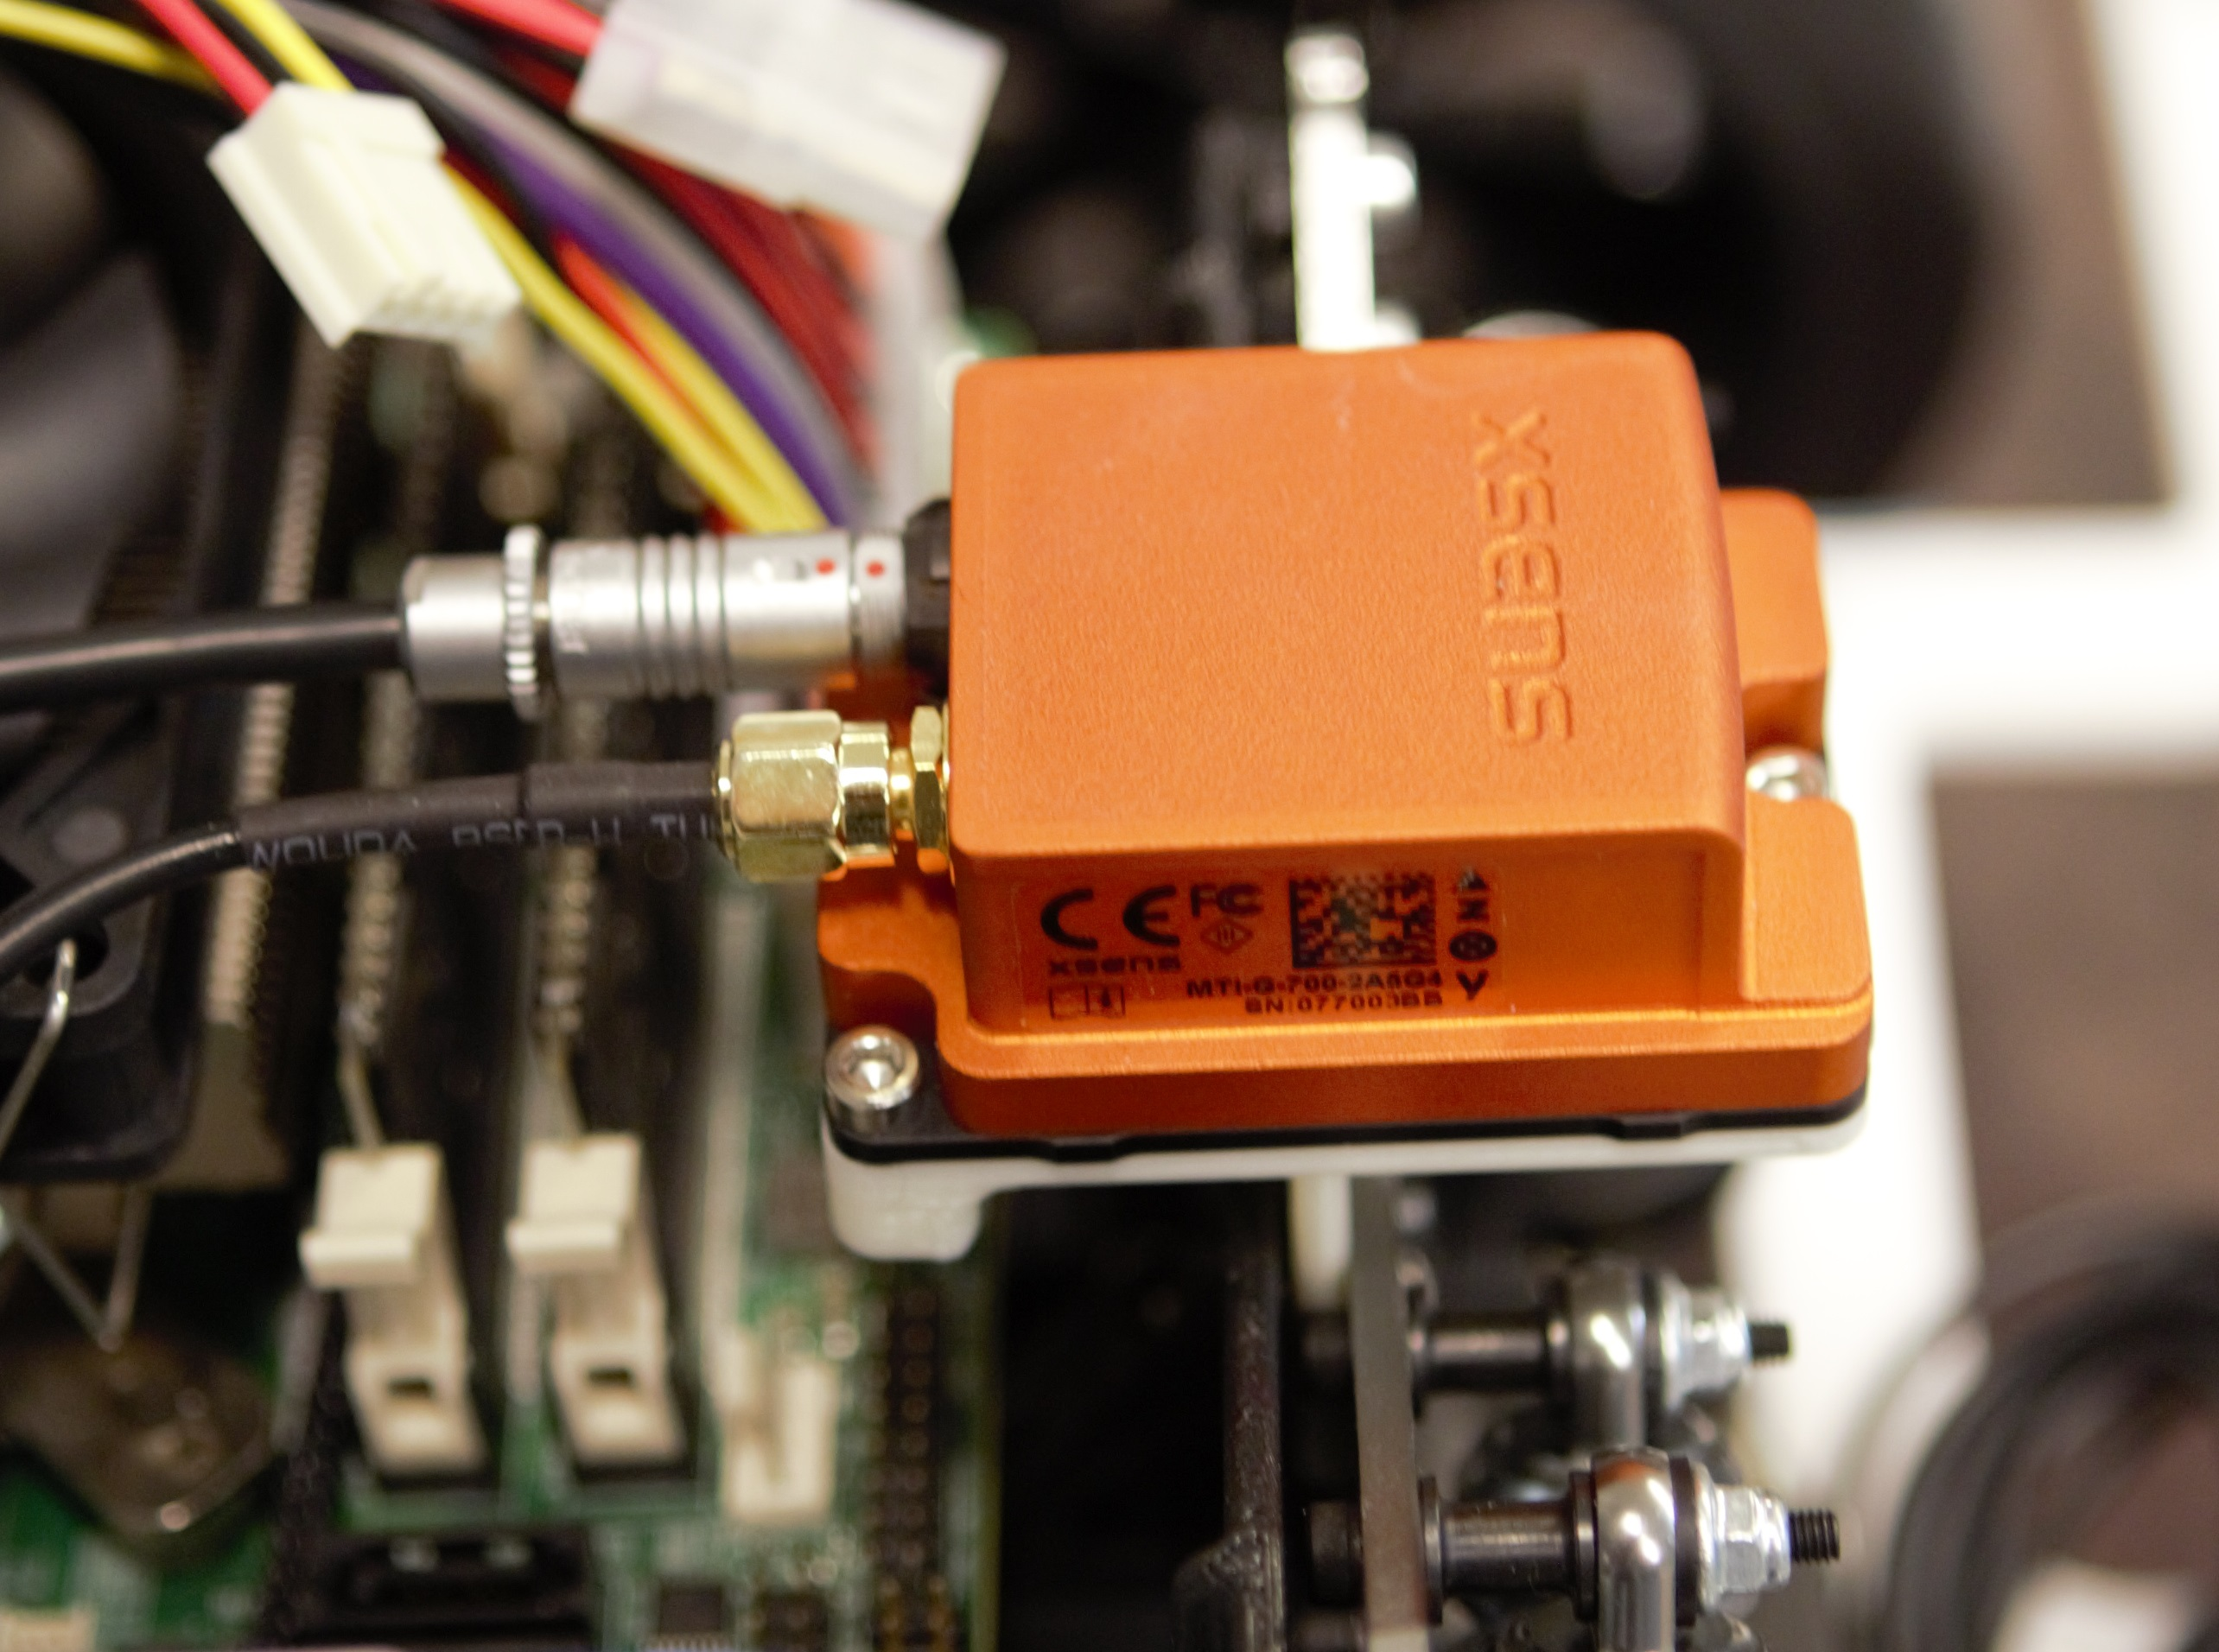
\includegraphics[width=0.4\textwidth]{xsens}
	\caption{XSens MTi-G-700}
	\label{fig:xsens}
\end{figure}

At the back of the car there is an X-Sens MTI-G-700 Inertial Measurement Unit (IMU). It contains sensors for accelerations in every spatial direction, for angle velocities and orientation about each axis and a GPS-module. Table \reftab{imu_details} gives some details of the module. For more information see: 

\hyperref[http://www.xsens.com/products/mti-g-700/]{http://www.xsens.com/products/mti-g-700/}

\begin{table}[h]
	\centering	
	\begin{tabular}{cc} % eine Tabelle mit drei Spalten, in denen der Text jeweils zentriert ist
		\hline 
		Name: & XSens MTi-G-700 \\
		Output frequency: & Up to 2000Hz \\
		Standard full range gyro: & 450 \textdegree/s \\
		Standard full range acc		& 50 m/s2 \\
		In-run bias stability gyro& 10 \textdegree/h \\
		\hline
	\end{tabular}
	\caption{IMU - Details} % Die Beschriftung der Tabelle
	\label{tab:imu_details}
\end{table}




%=========================================================================================
\section{Software}
%=========================================================================================
\label{sec:overview_software}

The operating system currently running on the linux board of the car is Ubuntu 14.04. To work with the hardware there is installed a software framework called Robot Operating System (ROS) which provides a big number of libraries and tools to work with robots. On the car we use the currently newest version: ROS Indigo \footnote{Since ROS Fuerte there are two different build systems. We use the catkin build system}. 

 At the beginning of the course you should get familiar with the functionality of ROS. A good start are the official tutorials on: 

\hyperref[http://wiki.ros.org/]{http://wiki.ros.org/}

After working with the tutorials you should understand the concept of nodes and topics and be able to create and build your own package. To work with the car there is a package on GitHub you can download and install on your system. See the next chapter for more information.


%=========================================================================================



